\chapter{Background}

In this chapter we will present concepts and existing tools relevant to this thesis. The first section presents \textit{Parallelization} and how it can be achieved in existing applications. Next we introduce \textit{Dynamic binary instrumentation} and how it can be used to analyze the runtime behavior of applications. Section 3 is a brief overview of \textit{SQLite}. Next we present \textit{Visualizations} and how they can be displayed in the browser. The last section presents \textit{Parceive}, a tool with which our implementation is compatible and is used to display the results of our analysis.

\section {Parallelization}

\subsection{Introduction}

Traditionally software has been designed for serial computation where instructions are executed one at a time on the same processor. Unfortunately single core performance in CPUs has stalled for the last 10 years as processor manufacturers focus on multi-core systems in order to increase overall performance \cite{procspeed2}.

Flynn has proposed a taxonomy \cite{flynn} to classify parallel hardware. \textbf{SIMD} allows instructions to operate on multiple data elements at the same time. \textbf{MISD} is an uncommon architecture where multiple processors operate on the same data. This thesis is focused on \textbf{MIMD} where each processor executes different instructions and can operate on data independently.

\subsection{Ahmdahl's Law}

Ahmdahl's Law \cite{amdahl} is a very coarse estimation for the possible speedup when running an application on multiple cores. The only parameters of the equation \ref{eq:ahmdahl} are $r_s$, the ratio of the sequential portions of the program, $n$, the number of processors, and $r_p$ the ratio of program code that can be run in parallel.

\begin{equation} \label{eq:ahmdahl}
	\begin{aligned}
		Speedup &= \frac{1}{r_s + \frac{r_p}{n}} \\
		r_s + r_p &= 1
	\end{aligned}
\end{equation}

More precise models have been proposed \cite{gustafson}, but in all of them it is clear that increasing performance requires more of the application to be executed in parallel.

\subsection{Steps to parallelize existing sequential software}

\begin{enumerate}[\hspace{80pt}(P1)]
	\item [Concurrency identification] A software developer or tool must determine what parts of the application can be run in parallel.
	\item [Architecture redefinition] The parallel execution model for the application must be chosen.
	\item [Parallelization] Implementing the Architecture.
	\item [Validation and Verification] Manual and automated testing verifies the correctness of the modifications.
	\item [Runtime analysis] The performance of the new system is evaluated
\end{enumerate}

This thesis is focused on the first step of parallelizing existing software. We provide a framework to evaluate the potential speedup and the feasibility of parallelizing parts of the application.

\subsection{Parallelization patterns}

This thesis focuses on two parallelization patterns, data parallelism and pipeline parallelism.

\subsubsection{Data parallelism}

Data parallelism \cite{parbook} focuses on distributing the processing across different processors by splitting up the data into chunks. This method is able to achieve scalability by generating more parallelism as the amount of data grows.

Data parallelism can be implemented using specialized instructions that operate on multiple items at the same time. This thesis focuses on thread parallelism where larger units of work are distributed across multiple processors.

Figure \ref{cap2:datapar} shows how a sequential processing of data can be distributed among multiple nodes.

\begin{figure}
	\centering
	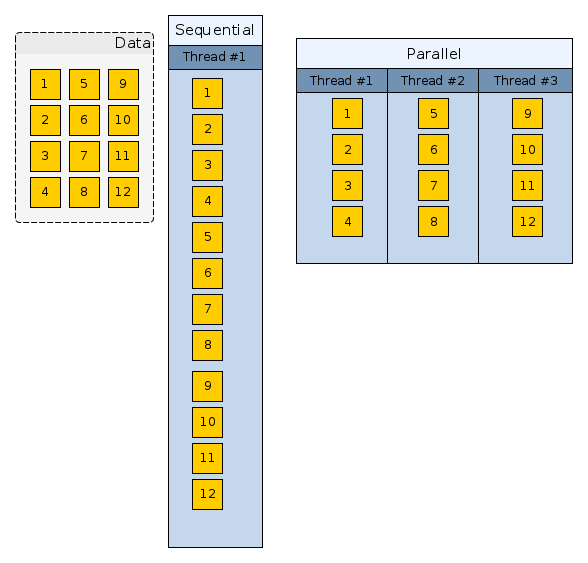
\includegraphics[width=1\textwidth]{seqtopar}
	\caption{Distributing work}
	\label{cap2:datapar}
\end{figure}

\subsubsection{Pipeline parallelism}

A pipeline \cite{parbook} is a linear sequence of processing stages that transform data. These stages must be applied in order, but the data can be split up into individual items and each item can be processed independently. As a simple example we consider file processing, where data is read, processed and written to another file. Individual iterations can not be run in parallel, but the io operations and the processing can be seen in Figure \ref{cap2:pipeline}.

\begin{figure}[!ht]
	\centering
	\begin{tabular}{ l | l | l | l | l}
		R & P & W & & \\
		\hline
		R &  & P & W & \\
		\hline
		R &  & & P & W \\
	\end{tabular}
	\caption{Pipeline, R - read, P - proecess, W - write}
	\label{cap2:pipeline}
\end{figure}

The speedup obtained by a pipeline is limited by the number of parallel stages that can be implemented. For the example in Figure \ref{cap2:pipeline} this is 3. Increasing the number of processors above this value will not provide any additional performance benefits.

\subsection{Dependencies}
\label{cap2:dependencies}

Sequential programs expect instructions to be executed in the order specified in the program. Parallelizing sections of programs violates this assumption and may cause unexpected behavior if the implicit dependencies between the tasks are not respected.

There are two kinds of dependencies for parallel code \cite{parbook}:

\textbf{Data dependencies} occur when an operation assumes that its inputs have been generated by a different task.

\textbf{Control dependencies} result when side effects (such as I/O Operations) need to be ordered.

Ensuring that dependencies do not cause issues requires synchronization between different tasks. Some sections of a program do not perform better when parallelized due to the number of dependencies between them. This limitaion makes it difficult to parallelize existing sequential applications.

\section {Dynamic Binary Instrumentation}

\subsection{Introduction}

Dynamic binary instrumentation is a method to analyze and alter the dynamic behavior of an application by modifying its instructions at runtime. This method makes it possible to gain insight into the state of a running program at any point in time and can also allow tools to alter that state. Dynamic binary instrumentation is used to follow a specific path trough an applications and is by no means exhaustive.

Most tools developed using this method are designed to obtain information about an application. For example MemTrace \cite{pindoc} and Memcheck \cite{memcheck} help discover and correct memory problems. Intel Advisor \cite{inteladvisor} and the tools described in this thesis aid in parallelization endevours.

Dynamic binary instrumentation can also be used to alter the state of a running program. Tools have implemented automatic fault injection \cite{faultinject}, dynamic transactional memory \cite{dynamicstm} and improvements to security \cite{dynamicstackprotect}.

\subsection{Implementations}

\subsubsection{Valgrind}

Valgrind \cite{valgrind} is an open-source dynamic binary instrumentation framework that is used to perform a number of powerful and diverse analyses. It focuses on using shadow values to implement complex tools, that are difficult to develop with other frameworks. Unfortunately even simple tools require a complex implementation and have a considerable overhead.

\subsubsection{Dyninst}

Dyninst \cite{dyninst} is a framework developed at the University of Maryland that performs dynamic binary instrumentation on a target application. The goal of this project is to abstract away machine code in order to create simple and portable tools. Multiple projects have taken advantage of Dyninst, for exaple VampirTrace \cite{vampirtrace}.

\subsubsection{Intel Pin}

Intel Pin \cite{pin} is a instrumentation framework that can be used to build a large variety of tools for Windows and Linux. The implementation is focused on ease-of-use and provides a very simple but powerful API that allows tools to instrument any instruction in a program.

\subsubsection{Example tools}

\emph{Memcheck} \cite{memcheck} is a tool developed as part of Valgrind that detects common C and C++ memory errors. It is able to report accesses to unallocated or uninitialized memory, incorrect usage of allocations or deallocations and memory leaks.

\emph{Intel Advisor} \cite{inteladvisor} is a collection of related tools based on Intel Pin that focus on helping developers parallelize applications. It is able to predict possible improvements when applying vectorisation and thread parallelism to applications.

\subsection{Overhead}

Unfortunately dynamic binary instrumentation entails a performance overhead when running programs. Valgrind for example runs programs 4.3x slower \cite{valgrind} even when not performing any kind of analysis. The slowdown becomes more substantial (22.1x) when executing a proper tool.

The overhead of the instrumentation can be split up in tow parts, modification of the target program and the execution of additional instructions. Tools such as Valgrind and Intel Pin also utilize a just-in-time virtual machine to execute the target, which creates an additional overhead. In \cite{instoverhead} there is a breakdown of time and instruction count when running an application with Intel Pin and performing an analysis.

\subsection{Alternatives}

Static analysis tools such as the Clang Static Analyser \cite{clang} or Coverity \cite{coverity} are able to identify potential faults in an application by inspecting its source code. This type of scrutiny considers all possible paths an application can potentially follow. This will detect problems in code that is rarely tested, but can also make it very computationally intensive. In contrast to this, dynamic analysis only follows a single path trough the application, but it can find many more issues with this one particular execution.

Code instrumentation tools such as the Intel Advisor \cite{inteladvisor} allow a software developer to insert instrumentations into the source code of the application. Running analyses on the application becomes a cycle of editing the source code, rebuilding and then running. This cycle can be too restrictive when working with an existing application that depends on a convoluted build process. Binary instrumentation works with the compiled application directly and does not require the developer to perform rebuilds.

Static binary instrumentation tools such as PEBIL \cite{pebil} alter an application executable by changing the instructions contained within. The new program can then be executed normally. This method can provide some performance benefits, but not in all cases as can be seen in \cite{pebilperf}. The drawback of these tools is the lack of flexibility when instrumenting as it is not possible to change instructions at runtime.

\subsection{Intel Pin}

The implementation of the tools presented in this thesis ares based on Intel Pin. This framework has been chosen because of the simple API, performance, good documentation and the flexibility when performing instrumentation.

\subsubsection{API}

The Pin API \cite{pindoc} simplifies the development of tools by providing two types of callbacks. Instrumentation routines are called when the tools must process parts of the target program. Analysis routines are the instrumentations that are called during the program execution. All routines are developed using standard C/C++ and can take advantage of any existing library.

Two of the most interesting instrumentation routines are trace callbacks and image callbacks. A image callback is called when the application or a shared library is loaded and allow the tool to instrument functions as they are detected in the executable code. A trace callback is called when the JIT compiler encounters new code and allows the tool to insert instrumentations into the instruction stream.

Instrumentation routines insert calls to analysis routines in order to acquire information or to modify the program state. Pin attempts to reduce the overhead of inserted code by automatically optimizing the analysis routines and the calling site.

The provided API allows a tool to perform a very granular analysis without the need to go trough a intermediate representation of the instruction stream. This greatly simplifies development and makes it possible to optimize the instrumentation.

\subsubsection{Documentation}

Intel Pin provides a comprehensive documentation \cite{pindoc} and a large number of examples as part of its distribution. The provided samples illustrate the different classes of tools that can be developed using the framework.

\subsubsection{Fast Buffers}

The Intel Pin Fast Buffering API \cite{pinbuffer} aims to decouple information collection from processing in order to reduce the overhead associated with dynamic binary instrumentation. This is implemented by collecting multiple chunks of data and processing them only when the buffer used to store them is full.

The greatest benefit of using the Intel Pin Fast Buffering API is the increased performance when performing analyses on applications \cite{pinbuffer}. This comes at the cost of being unable to alter the application state during execution. The tools developed as part of this thesis need to change the application behavior and are implemented using this API.

The provided API is similar to the standard Pin API \cite{pindoc}. Instrumentation routines remain unchanged, but it is not possible to insert instrumentations into the program outside trace instrumentation. Buffer allocation and management is performed automatically by Pin and the tool only needs to define a buffer with a callback to handle the data processing. Information gathering is performed by instrumentation code generated by Pin and can examine any aspect of the application state.

\section{SQLite}

SQLite \cite{sqlitebook} is an open-source relational database management system that does not require a server. It is implemented as a self-contained library that supports most features of the SQL92 standard.

In contrast to traditional RDBMS, SQLite is not based on a client/server architecture. Its entire engine is integrated into the application that accesses or manipulates the database. This reduces the footprint and complexity of a system that incorporates SQLite instead of a server.

SQLite stores the entire database in a single file. This file contains the schema, all data stored in tables and indexes. The storage format is platform agnostic which allows easy backup and sharing of an entire database.

Compared to writing a text file using the standard library SQLite is between 30-50\% faster. This performance is achieved by a release build of a Intel Pin tool when writing to a database without indexes and by disabling journaling running on our setup described in Appendix \ref{appendix:setup}.

Parceive and the tools implemented as part of this thesis store data as a SQLite database. This allows results of an application trace to be easily manipulated, while maintaining a high degree of performance. Additional analysis can be easily performed on the database by using standard SQL statements, as will be presented in Section \ref{dataprocessing}.

\section {Visualizations}

Gathering large amounts of data about an applications does not benefit an user if it can not be navigated or condensed into an useful form. A graphic representation makes the information accessible and allows an user to reason about it.

\subsection {SVG}

SVG \cite{svg11} is a vector image format based on XML designed for two-dimensional graphics based on an open web standard. It can be easily integrated into HTML and supports interactivity and complex animations. Since 2011 most browsers implement native support for SVG.

Many visualization frameworks have been developed to work with SVG inside browsers such as D3, Vega, Processing or dygraphs. The standard provides all primitives required to implement any kind of 2D visualization. Interactivity and animations are possible with javascript as SVG documents are part of the Document Object Model.

The most important features of SVG used by visualizations are:

\begin{itemize}
	\item[Paths] allow arbitrary shapes to be defined
	\item[Basic shapes] such as lines, circles and rectangles
	\item[Text elements] make it easy to insert text in a visualization
	\item[Groups] allow easy and efficient manipulation of multiple elements
	\item[Interactivity] implemented with the use of events and the DOM
	\item[Animations] possible with CSS, Javascript or built-in elements
	\item[Linking] allows references to other parts of the document
\end{itemize}

\section{Parceive}
\label{cap2:parceve}

Parceive \cite{parceive} is a tracing-based tool for parallelizing existing sequential software. It focuses on high-level architecture analysis, but also gathers fine-grained memory accesses and call information.

\subsection{Architecture}

In Figure \ref{parceive:architecture} we can see the overall architecture of the Parceive project. Parceive is based on Intel Pin and is designed to store a trace of the application in a SQLite database. This database is then processed to improve the performance of visualizations that access information from it. A simple NodeJS acts as a bridge between the browser and the database. Views access data using a Object Relational Mapping that performs multiple optimizations to improve throughput. The visualization framework organizes the display of visualizations on the page and implements state management.

\begin{figure}
	\centering
	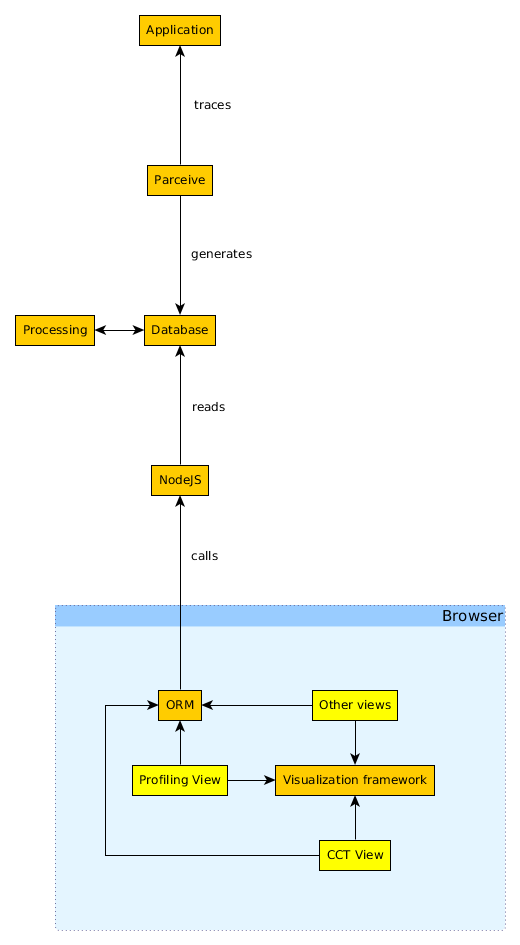
\includegraphics[width=0.6\textwidth]{parceive}
	
	\caption{Parceive architecture}
	\label{parceive:architecture}
\end{figure}

\subsection{Pin tool}

Parceive is the data gathering component of the project. It traces the run of an application and stores its the function calls, memory accesses and loop executions in a SQLite database. The size of the result can be reduced by applying filters at the image, source file and function level.

This tool also performs variable name resolution using DWARF or DebugHelp information present in the executable. This greatly improves the quality of the information available to visualizations.

\subsection{Database layout}

The database layout used by Parceive is closely related to the entities available in the Pin API and is very simple as can be see in Figure \ref{parceive:layout}. In this section we will briefly explain what each table contains and how entities are related to each other.

An Image is the program executable or a shared library loaded by it and can contain multiple functions and source files. The Call table contains information about all the function calls made by the application. A call consists of multiple segments which contain actual instructions. Segments are used to indicate loops inside calls. If a segment is part of a loop a corresponding LoopIteration entry exists to store details. Loop iterations are grouped into loop executions to make it possible to differentiate the loop instances. Static information about loops is stored in the Loop table

Instructions are only stored when they access memory, call a function, create a thread or allocate memory. A instruction can access multiple memeory locations and in different ways. The Reference table contains interesting memory slices and is populated using debug information or allocations. Currently arrays are stored as a single reference.

\begin{sidewaysfigure}
	\centering
	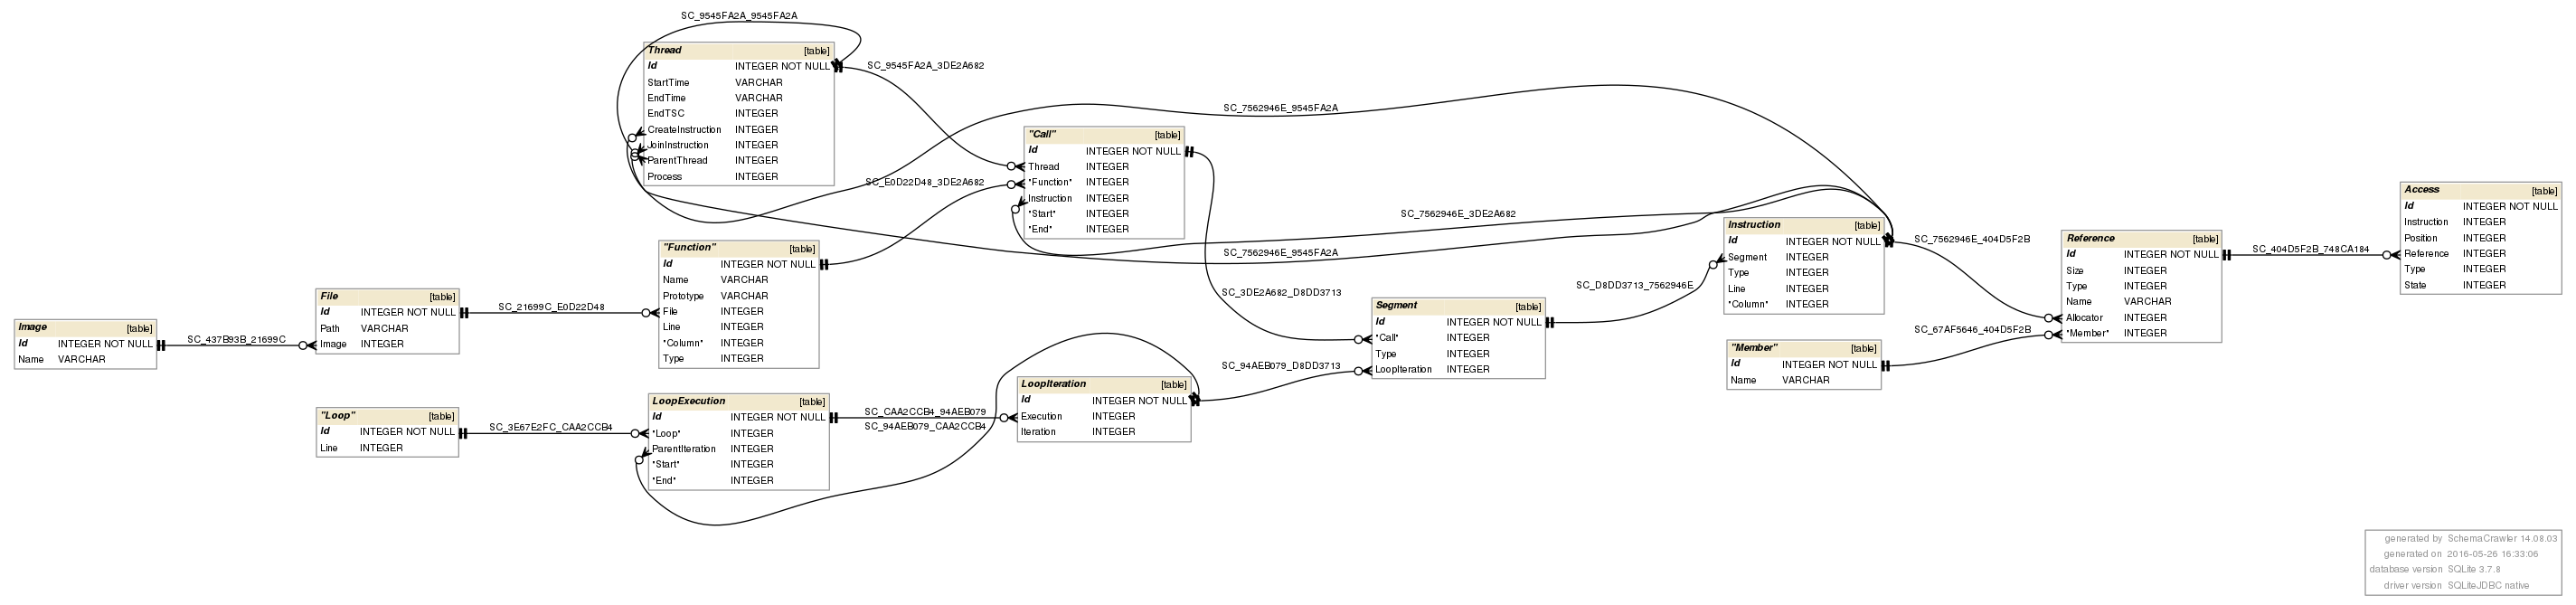
\includegraphics[width=1\textwidth]{parceive-schema}
	\caption{Parceive database layout}
	\label{parceive:layout}
\end{sidewaysfigure}

\subsection{Database processing}
\label{dataprocessing}

The database layout and settings used by Parceive are highly optimized for writing. All the trace data required by the visualization can be obtained by using queries, but most of the operations will take a disproportionate amount of time to complete.

The first problem with databases optimized for writing is the lack of indexes. Thus, the most important step of the database processing is the creation of multiple indexes to improve record lookup. All primary and foreign keys are indexed and some composite indexes are created to speed up queries that perform poorly.

The data requested by visualizations requires joins across three or more tables and did not perform well. By adding additional fields and creating intermediary tables, it is possible to avoid joins for most queries executed by the visualizations. Since no additional data will be added to the database, creating redundancy generates no runtime overhead and does not increase the complexity.

Trace databases that are not created by inserting entries in order and become very fragmented. Executing \texttt{VACUUM}, a SQL statement, after all processing is completed eliminates this problem. The increased locality of data reduces the execution time of most queries and has a considerable effect on ones that require a full table scan. \texttt{VACUUM} is also able to reduce the size of the processed database.

The structure of a processed database can be see in Figure \ref{parceive:proclayout}.

\subsubsection{Optimization examples}

1. One of the most intuitive and beneficial information added to the database is the \texttt{Caller} field in the \texttt{Call} table. Obtaining the calls performed by one specific call normally requires a join on three tables \texttt{Call}, \texttt{Instruction} and \texttt{Segment} and can be completely avoided by this shortcut.

2. Showing profiling information of a call would require querying all calls made. If loops are present most of the calls would be made to the same function. The creation of the \texttt{CallGroup} table reduces the number of entities returned considerably by grouping together all calls to the same function. A profiler can avoid the \texttt{Call} table completely by using \texttt{CallGroup}.

3. SQL is not designed to handle tree structures such as the call graph present in an application. The \texttt{CallTree} and \texttt{CallGroupTree} tables contain a flattened representation of the graph that can be queried in a simple and readable manner. Complex queries only become possible by using of these intermediary tables. The following queries would require hours of processing time if not optimized:

\begin{itemize}
	\item The references accessed during the execution of a call
	\item Loading an entire call graph at once
\end{itemize}

\subsubsection{Performance}

Figure \ref{parceive:procperformance} shows the time and size overhead of processing databases generated by Parceive. The time required by this operation is negligible because loading most visualizations without the optimizations would waste more than the processing itself. The executed queries are also heavily optimized making \texttt{VACUUM} and the creation of indexes the most time consuming operations.

\begin{figure}
	\centering
	\begin{tabular}{l l l l}
		Database & Size & Processed Size & Time taken \\
		emsim\_par & 3905536 & 14560256 & 8.77 s
	\end{tabular}
	\caption{Database processing performance}
	\label{parceive:procperformance}
\end{figure}

\begin{sidewaysfigure}
	\centering
	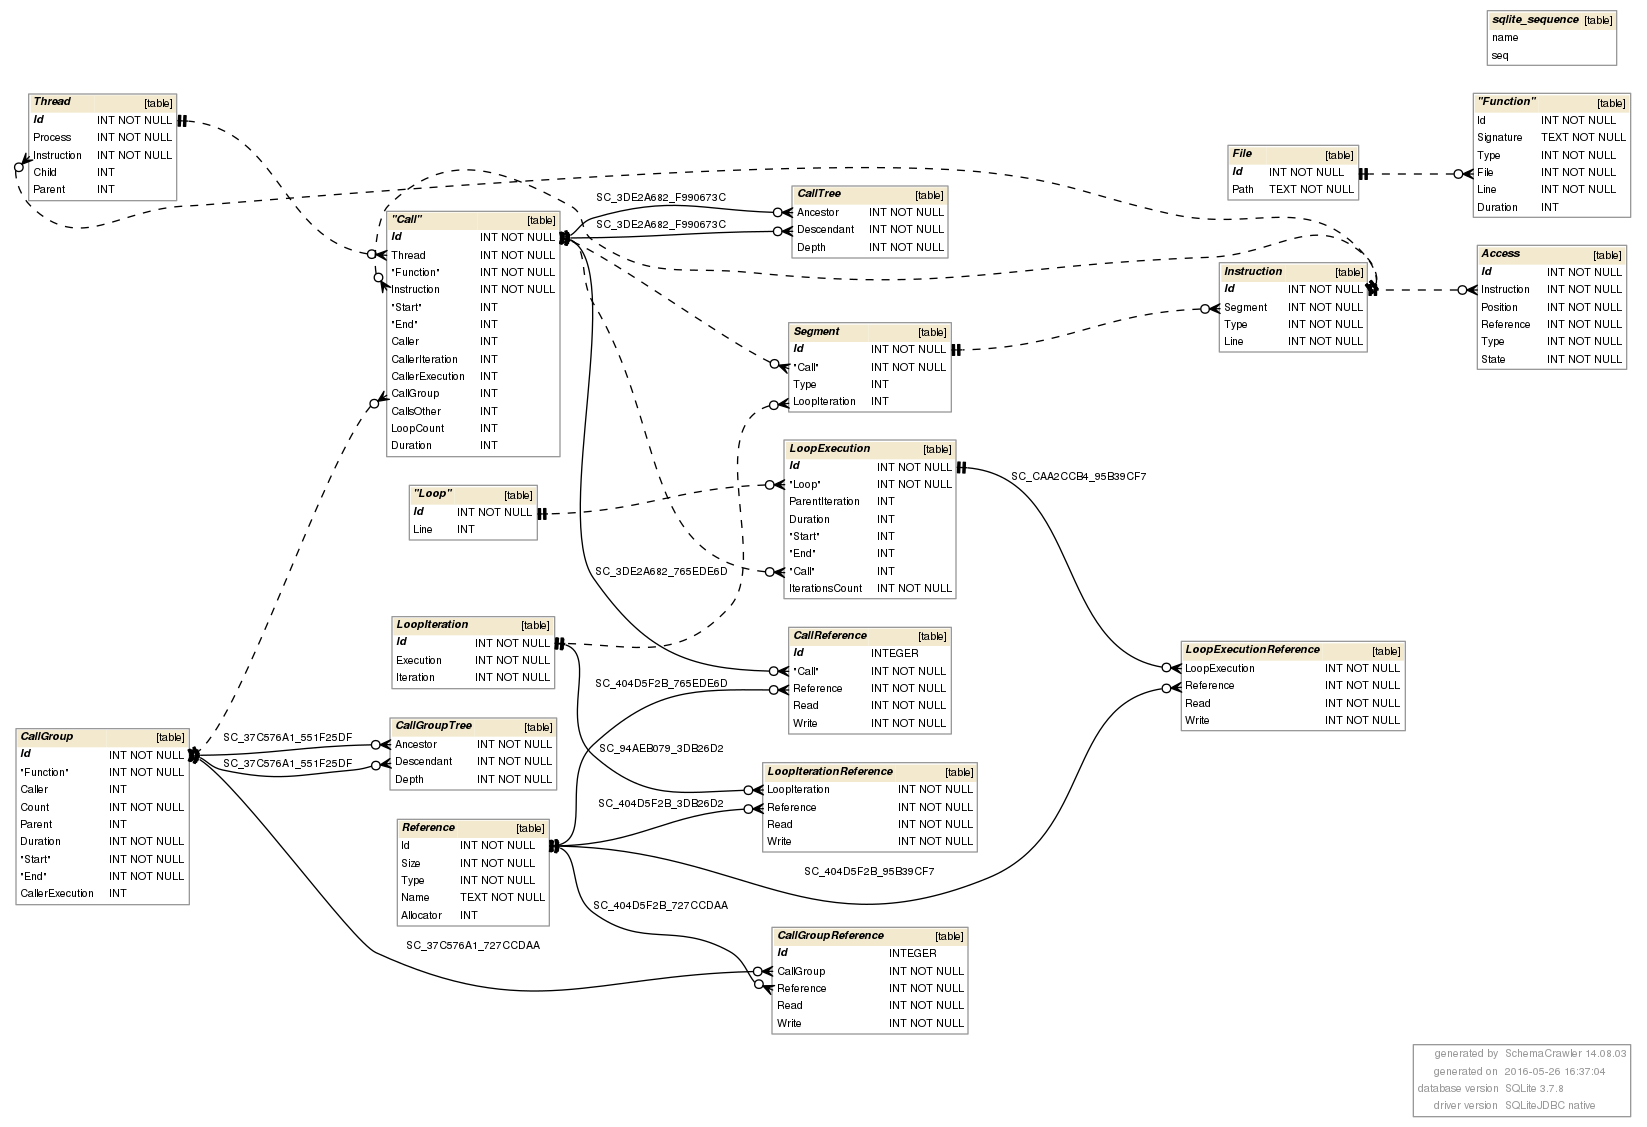
\includegraphics[width=0.8\textwidth]{full-schema}
	\caption{Processed database layout}
	\label{parceive:proclayout}
\end{sidewaysfigure}

\subsection{NodeJS Server}

Loading large trace databases into current browsers may exceed their memory restrictions. To solve this problem a simple NodeJS Server was developed hat reads data from a processed database on demand.

The server exposes a REST \cite{rest} API for the retrieval of data. For security reasons all SQL queries are integrated in this server without support for arbitrary queries. The implementation makes use of multiple parallel reads to the same database to reduce the latency and throughput when large amounts of data is requested by the visualizations.

\subsection{ORM}

Visualizations developed within the Parceive architecture can employ an Object Relational Mapper to simplify development and improve performance. The ORM makes it ossible to access entities and to easily navigate the relationships between them. The API is implemented using promises \cite{promises} simplifying the asynchronous and parallel behavior.

The greatest benefit of using this ORM in views is the possibility of applying optimizations to the data loading. The most important ones are caching and pipelining.

Caching allows the ORM to avoid loading data that has been accessed before. Each time an entity is retrieved from the server it is saved and reused for subsequent requests. This optimization allows the views to focus on data presentation instead of efficient data retrieval.

Pipelining combines multiple queries to the same REST API call into a single one. When requesting a large number of entities this approach improves performance despite the limit on the number of parallel requests in browsers. This optimization is designed to greatly increase throughput at the cost of an increased response time.

\subsection{Visualization Framework}

As part of the Parceive UI a visualization framework has been developed to handle the layout and communication of multiple visualizations. The implementation is based on AngularJS and it completely separates visualizations into separate applications.

\subsubsection{Communication}

Visualizations allow the user to navigate the callgraph in different ways. Communication makes it possible to follow a chain of investigation along multiple visualizations. Currently there are three ways to communicate intent:

\begin{itemize}
	\item[Focus] brings entities to the attention of the user
	\item[Mark] allows the creation of selections that are visible between visualizations
	\item[Spot] replaces all the entities in a visualization with a new set
	\item[Hover] brings entities to the attention of the user using opacity
\end{itemize}

\subsubsection{State management}

The visualization framework also implements a centralized and persistent state management for visualizations. With the use of this feature it is possible to retain the state of views across page views.

Currently the view layout and the marked nodes are stored as part of the state automatically. In addition to this each visualization can save tailored information at any time and retrieve it when rendering. Local storage is used to house all the state information making it persistent.

\subsubsection{API}
Each visualization is an AngularJS application and isolated from the others. The Visualization Framework is able to detect such applications by a special naming scheme and the interface they provide. A visualization must provide the following functions:

\subsubsection{Communication}

Views allow the user to navigate the callgraph in different ways. Communication makes it possible to follow a chain of investigation along multiple visualizations. Currently there are three ways to communicate intent:

\textbf{Focus} brings entities to the attention of the user

\textbf{Mark} allows the creation of selections that are visible between visualizations

\textbf{Spot} replaces all the entities in a visualization with a new set

\textbf{Hover} brings entities to the attention of the user using opacity